% Select document class: uncomment one of the following
\documentclass[aspectratio=169]{beamer}  % For presentation mode
%\documentclass[11pt]{article}            % For article mode
%\usepackage{beamerarticle}               % Uncomment with article class

% =============================================================================
% COMMON PREAMBLE
% =============================================================================
% =============================================================================
% Common Preamble for Network+ Lecture Series
% This file provides consistent formatting, colors, packages, and styles
% across all lecture modules for both beamer presentations and article mode
% =============================================================================

% =============================================================================
% THEME AND COLORS
% =============================================================================
\usetheme{Madrid}
\usecolortheme{whale}

% Custom colors - standardized across all lectures
\definecolor{rctcblue}{RGB}{0, 74, 136}
\definecolor{rctcgold}{RGB}{255, 199, 44}
\definecolor{networkgreen}{RGB}{0, 128, 64}
\definecolor{alertred}{RGB}{180, 0, 0}
\definecolor{aborange}{RGB}{230, 126, 34}
\definecolor{copperbrown}{RGB}{184, 115, 51}
\definecolor{faborange}{RGB}{255, 165, 0}
\definecolor{fiberyellow}{RGB}{255, 215, 0}
\definecolor{shirepurple}{RGB}{102, 51, 153}
\definecolor{ipblue}{RGB}{52, 152, 219}
\definecolor{ippurple}{RGB}{155, 89, 182}
\definecolor{vlangreen}{RGB}{39, 174, 96}
\definecolor{tcpblue}{RGB}{30, 100, 180}
\definecolor{udpgreen}{RGB}{50, 160, 80}
\definecolor{dhcppurple}{RGB}{120, 60, 160}
\definecolor{dnsyellow}{RGB}{200, 170, 50}
\definecolor{batblack}{RGB}{30, 30, 40}
\definecolor{gothamgray}{RGB}{80, 85, 95}
\definecolor{paddysgreen}{RGB}{19, 77, 33}
\definecolor{beerlight}{RGB}{255, 199, 44}
\definecolor{sunnyorange}{RGB}{255, 140, 0}
\definecolor{ogregreen}{RGB}{34, 139, 34}
\definecolor{swampbrown}{RGB}{101, 67, 33}

% Set theme colors
\setbeamercolor{palette primary}{bg=rctcblue,fg=white}
\setbeamercolor{palette secondary}{bg=rctcblue!80,fg=white}
\setbeamercolor{palette tertiary}{bg=rctcblue!60,fg=white}
\setbeamercolor{structure}{fg=rctcblue}
\setbeamercolor{title}{fg=white,bg=rctcblue}
\setbeamercolor{frametitle}{fg=white,bg=rctcblue}
\setbeamercolor{block title}{bg=rctcblue,fg=white}
\setbeamercolor{block body}{bg=rctcblue!10,fg=black}
\setbeamercolor{block title alerted}{bg=alertred,fg=white}
\setbeamercolor{block body alerted}{bg=alertred!10,fg=black}
\setbeamercolor{block title example}{bg=networkgreen,fg=white}
\setbeamercolor{block body example}{bg=networkgreen!10,fg=black}

% =============================================================================
% PACKAGES
% =============================================================================
\usepackage[utf8]{inputenc}
\usepackage[T1]{fontenc}
\usepackage{lmodern}  % Better font rendering
\usepackage{graphicx}
\usepackage{tikz}
\usepackage{booktabs}
\usepackage{array}
\usepackage{multirow}
\usepackage{hyperref}
\usepackage{adjustbox}
\usepackage{amssymb}
\usepackage{amsmath}
\usepackage{calc}
\usepackage{fontawesome5}
% xcolor with [table] option: avoid colortbl.4ht hook conflict in tex4ht
\ifdefined\HCode
  \usepackage{xcolor}
  \usepackage{colortbl}  % provides \rowcolor etc.
\else
  \usepackage[table]{xcolor}  % includes colortbl for pdflatex
\fi

% =============================================================================
% TIKZ LIBRARIES AND SETUP
% =============================================================================
\usetikzlibrary{
    shapes.geometric,
    shapes.symbols,
    shapes.misc,
    arrows.meta,
    positioning,
    calc,
    fit,
    backgrounds,
    decorations.pathreplacing,
    decorations.pathmorphing,
    matrix,
    chains
}
% shadows library causes pgfuseshading errors with tex4ht;
% only load it when NOT building HTML
\ifdefined\HCode\else
    \usetikzlibrary{shadows}
\fi

% Graphics path for icons and chapter images
\graphicspath{
    {../images/icons/}
    {./images/icons/}
    {images/icons/}
    {../images/ch1/}
    {./images/ch1/}
    {images/ch1/}
    {../images/ch2/}
    {./images/ch2/}
    {images/ch2/}
    {../images/ch3/}
    {./images/ch3/}
    {images/ch3/}
    {../images/ch4/}
    {./images/ch4/}
    {images/ch4/}
    {../images/ch5/}
    {./images/ch5/}
    {images/ch5/}
    {../images/ch6/}
    {./images/ch6/}
    {images/ch6/}
    {../images/ch7/}
    {./images/ch7/}
    {images/ch7/}
    {../images/ch8/}
    {./images/ch8/}
    {images/ch8/}
    {../images/ch9/}
    {./images/ch9/}
    {images/ch9/}
    {../images/}
    {./images/}
    {images/}
}

% =============================================================================
% NETWORK DIAGRAM STYLES
% =============================================================================
\tikzset{
    % Node styles for network devices
    device/.style={
        inner sep=2pt,
        label distance=2pt
    },
    pc/.style={device},
    laptop/.style={device},
    server/.style={device},
    router/.style={device},
    switch/.style={device},
    firewall/.style={device},
    cloud/.style={device},
    phone/.style={device},
    tablet/.style={device},
    wifi/.style={device},
    % Connection styles
    ethernet/.style={
        draw=rctcblue,
        line width=1.5pt,
        -{Stealth[length=3mm]}
    },
    ethernet noarrow/.style={
        draw=rctcblue,
        line width=1.5pt
    },
    wireless/.style={
        draw=aborange,
        line width=1.5pt,
        dashed,
        -{Stealth[length=3mm]}
    },
    wireless noarrow/.style={
        draw=aborange,
        line width=1.5pt,
        dashed
    },
    wan/.style={
        draw=alertred,
        line width=2pt,
        -{Stealth[length=3mm]}
    },
    wan noarrow/.style={
        draw=alertred,
        line width=2pt
    },
    copper/.style={
        draw=copperbrown,
        line width=2pt,
        -{Stealth[length=3mm]}
    },
    copper noarrow/.style={
        draw=copperbrown,
        line width=2pt
    },
    fiber/.style={
        draw=fiberyellow,
        line width=2pt,
        -{Stealth[length=3mm]}
    },
    fiber noarrow/.style={
        draw=fiberyellow,
        line width=2pt
    },
    trunk/.style={
        draw=shirepurple,
        line width=2pt,
        -{Stealth[length=3mm]}
    },
    trunk noarrow/.style={
        draw=shirepurple,
        line width=2pt
    },
    % Packet/segment styles
    pktseg/.style={
        draw=rctcblue,
        fill=rctcblue!10,
        minimum height=0.5cm,
        font=\tiny,
        rounded corners=2pt
    },
    pktseg tcp/.style={
        draw=tcpblue,
        fill=tcpblue!15,
        minimum height=0.5cm,
        font=\tiny,
        rounded corners=2pt
    },
    pktseg udp/.style={
        draw=udpgreen,
        fill=udpgreen!15,
        minimum height=0.5cm,
        font=\tiny,
        rounded corners=2pt
    },
    pktseg highlight/.style={
        draw=aborange,
        fill=aborange!20,
        minimum height=0.5cm,
        font=\tiny,
        rounded corners=2pt
    },
    % Box styles
    ipbox/.style={
        draw=rctcblue,
        fill=rctcblue!10,
        rounded corners,
        minimum height=0.4cm,
        font=\small
    },
    portbox/.style={
        draw=tcpblue,
        fill=tcpblue!10,
        rounded corners,
        minimum height=0.4cm,
        font=\small
    },
    dnsbox/.style={
        draw=dnsyellow,
        fill=dnsyellow!15,
        rounded corners,
        minimum height=0.4cm,
        font=\small
    },
    routetable/.style={
        draw=rctcblue,
        fill=rctcblue!10,
        rounded corners,
        minimum height=0.4cm,
        font=\small
    },
    macbox/.style={
        draw=networkgreen,
        fill=networkgreen!10,
        rounded corners,
        minimum height=0.4cm,
        font=\small
    },
    % Frame segment styles (Ethernet frame diagrams)
    frameseg/.style={
        draw=rctcblue,
        fill=rctcblue!10,
        minimum height=0.5cm,
        font=\tiny,
        rounded corners=2pt
    },
    frameseg highlight/.style={
        draw=aborange,
        fill=aborange!20,
        minimum height=0.5cm,
        font=\tiny,
        rounded corners=2pt
    },
    % Process/flow styles
    process/.style={
        draw=rctcblue,
        fill=rctcblue!15,
        rounded corners,
        minimum width=2cm,
        minimum height=0.6cm,
        font=\small,
        align=center
    },
    decision/.style={
        draw=aborange,
        fill=aborange!15,
        diamond,
        aspect=2,
        minimum width=1.5cm,
        font=\small,
        align=center
    },
    % OSI Layer styles
    osilayer/.style={
        draw=rctcblue,
        fill=rctcblue!10,
        minimum width=3cm,
        minimum height=0.45cm,
        font=\small
    },
    osilayer highlight/.style={
        draw=aborange,
        fill=aborange!20,
        line width=1.5pt,
        minimum width=3cm,
        minimum height=0.45cm,
        font=\small\bfseries
    }
}

% =============================================================================
% ICON COMMANDS - Standardized using PNG files and FontAwesome
% =============================================================================
% Network device icons (PNG)
\newcommand{\iconpc}[1][0.6cm]{\resizebox{#1}{!}{
\includegraphics{icon_pc}}}
\newcommand{\iconlaptop}[1][0.6cm]{\resizebox{#1}{!}{
\includegraphics{icon_laptop}}}
\newcommand{\iconserver}[1][0.6cm]{\resizebox{#1}{!}{
\includegraphics{icon_server}}}
\newcommand{\iconrouter}[1][0.6cm]{\resizebox{#1}{!}{
\includegraphics{icon_router}}}
\newcommand{\iconswitch}[1][0.6cm]{\resizebox{#1}{!}{
\includegraphics{icon_switch}}}
\newcommand{\iconfirewall}[1][0.6cm]{\resizebox{#1}{!}{
\includegraphics{icon_firewall}}}
\newcommand{\iconcloud}[1][0.6cm]{\resizebox{#1}{!}{
\includegraphics{icon_cloud}}}
\newcommand{\iconphone}[1][0.6cm]{\resizebox{#1}{!}{
\includegraphics{icon_phone}}}
\newcommand{\icontablet}[1][0.6cm]{\resizebox{#1}{!}{
\includegraphics{icon_tablet}}}
\newcommand{\iconwifi}[1][0.6cm]{\resizebox{#1}{!}{
\includegraphics{icon_wifi}}}
\newcommand{\icondatabase}[1][0.6cm]{\resizebox{#1}{!}{
\includegraphics{icon_db}}}
\newcommand{\iconlock}[1][0.6cm]{\resizebox{#1}{!}{
\includegraphics{icon_lock}}}

% For HTML/tex4ht builds: replace PNG icons with FontAwesome5 glyphs.
% dvisvgm embeds font glyphs as vectors but silently ignores em:graph (PNG)
% specials, so PNG icons would be blank in the output SVGs. FA5 glyphs work.
\ifdefined\HCode
  \renewcommand{\iconpc}[1][0.6cm]{\resizebox{#1}{!}{\faIcon{desktop}}}
  \renewcommand{\iconlaptop}[1][0.6cm]{\resizebox{#1}{!}{\faIcon{laptop}}}
  \renewcommand{\iconserver}[1][0.6cm]{\resizebox{#1}{!}{\faIcon{server}}}
  \renewcommand{\iconrouter}[1][0.6cm]{\resizebox{#1}{!}{\faIcon{route}}}
  \renewcommand{\iconswitch}[1][0.6cm]{\resizebox{#1}{!}{\faIcon{network-wired}}}
  \renewcommand{\iconfirewall}[1][0.6cm]{\resizebox{#1}{!}{\faIcon{shield-alt}}}
  \renewcommand{\iconcloud}[1][0.6cm]{\resizebox{#1}{!}{\faIcon{cloud}}}
  \renewcommand{\iconphone}[1][0.6cm]{\resizebox{#1}{!}{\faIcon{mobile-alt}}}
  \renewcommand{\icontablet}[1][0.6cm]{\resizebox{#1}{!}{\faIcon{tablet-alt}}}
  \renewcommand{\iconwifi}[1][0.6cm]{\resizebox{#1}{!}{\faIcon{wifi}}}
  \renewcommand{\icondatabase}[1][0.6cm]{\resizebox{#1}{!}{\faIcon{database}}}
  \renewcommand{\iconlock}[1][0.6cm]{\resizebox{#1}{!}{\faIcon{lock}}}
\fi

% FontAwesome icons
\newcommand{\iconuser}[1][0.6cm]{\resizebox{#1}{!}{\faIcon{user}}}
\newcommand{\iconglobe}[1][0.6cm]{\resizebox{#1}{!}{\faIcon{globe}}}
\newcommand{\iconclock}[1][0.6cm]{\resizebox{#1}{!}{\faIcon{clock}}}
\newcommand{\iconmail}[1][0.6cm]{\resizebox{#1}{!}{\faIcon{envelope}}}
\newcommand{\icondoc}[1][0.6cm]{\resizebox{#1}{!}{\faIcon{file-alt}}}
\newcommand{\iconsearch}[1][0.6cm]{\resizebox{#1}{!}{\faIcon{search}}}
\newcommand{\icontools}[1][0.6cm]{\resizebox{#1}{!}{\faIcon{tools}}}
\newcommand{\iconchart}[1][0.6cm]{\resizebox{#1}{!}{\faIcon{chart-line}}}
\newcommand{\iconalert}[1][0.6cm]{\resizebox{#1}{!}{\faIcon{bell}}}
\newcommand{\iconlog}[1][0.6cm]{\resizebox{#1}{!}{\faIcon{clipboard-list}}}
\newcommand{\iconeye}[1][0.6cm]{\resizebox{#1}{!}{\faIcon{eye}}}
\newcommand{\iconhacker}[1][0.6cm]{\resizebox{#1}{!}{\faIcon{user-secret}}}
\newcommand{\iconkey}[1][0.6cm]{\resizebox{#1}{!}{\faIcon{key}}}
\newcommand{\iconfile}[1][0.6cm]{\resizebox{#1}{!}{\faIcon{file-alt}}}
\newcommand{\icondog}[1][0.6cm]{\resizebox{#1}{!}{\faIcon{dog}}}
\newcommand{\iconcat}[1][0.6cm]{\resizebox{#1}{!}{\faIcon{cat}}}
\newcommand{\iconvoip}[1][0.6cm]{\resizebox{#1}{!}{\faIcon{phone-volume}}}
\newcommand{\iconmoney}[1][0.6cm]{\resizebox{#1}{!}{\faIcon{money-bill-wave}}}
\newcommand{\icontrash}[1][0.6cm]{\resizebox{#1}{!}{\faIcon{trash}}}
\newcommand{\iconbuilding}[1][0.6cm]{\resizebox{#1}{!}{\faIcon{building}}}

% =============================================================================
% CUSTOM COMMANDS AND ENVIRONMENTS
% =============================================================================

% Key term formatting
\newcommand{\keyterm}[1]{\textbf{#1}}

% Slide section marker
\newcommand{\sectionslide}[1]{
    \begin{frame}
        \vfill
        \centering
        \begin{beamercolorbox}[sep=8pt,center,shadow=true,rounded=true]{title}
            \usebeamerfont{title}\Huge #1
        \end{beamercolorbox}
        \vfill
    \end{frame}
}

% Case study frame environment
\newenvironment{casestudy}[1]{%
    \begin{alertblock}{$\blacktriangleright$ Case Study: #1}
}{%
    \end{alertblock}
}

% Solution frame environment  
\newenvironment{casesolution}[1]{%
    \begin{exampleblock}{$\checkmark$ Solution: #1}
}{%
    \end{exampleblock}
}

% =============================================================================
% FOOTER WITH SLIDE NUMBERS
% =============================================================================
\setbeamertemplate{footline}{
    \leavevmode%
    \hbox{%
        \begin{beamercolorbox}[wd=.333333\paperwidth,ht=2.25ex,dp=1ex,center]{author in head/foot}%
            \usebeamerfont{author in head/foot}\insertshortauthor
        \end{beamercolorbox}%
        \begin{beamercolorbox}[wd=.333333\paperwidth,ht=2.25ex,dp=1ex,center]{title in head/foot}%
            \usebeamerfont{title in head/foot}\insertshorttitle
        \end{beamercolorbox}%
        \begin{beamercolorbox}[wd=.333333\paperwidth,ht=2.25ex,dp=1ex,right]{date in head/foot}%
            \usebeamerfont{date in head/foot}\insertshortdate{}\hspace*{2em}
            \insertframenumber{} / \inserttotalframenumber\hspace*{2ex}
        \end{beamercolorbox}}%
    \vskip0pt%
}

% =============================================================================
% ARTICLE MODE SUPPORT
% =============================================================================
% The following commands help with beamerarticle mode for HTML conversion

% In article mode, add proper section/subsection support and override environments
\mode<article>{
    % Make sure figure captions work properly
    \setbeamertemplate{caption}[numbered]
    \setbeamertemplate{caption label separator}{: }
    
    % Add some spacing for readability
    \setlength{\parskip}{0.5em}
    \setlength{\parindent}{0pt}
    
    % Article mode versions of case study environments
    \renewenvironment{casestudy}[1]{%
        \vspace{0.3cm}\noindent\textbf{Case Study: #1}\newline\begin{itshape}
    }{%
        \end{itshape}\vspace{0.3cm}
    }
    
    \renewenvironment{casesolution}[1]{%
        \vspace{0.3cm}\noindent\textbf{Solution: #1}\newline\begin{itshape}
    }{%
        \end{itshape}\vspace{0.3cm}
    }
}

% Command to mark content that only appears in article mode
\newcommand{\articleonly}[1]{\mode<article>{#1}}

% Command to mark content that only appears in presentation mode
\newcommand{\presentationonly}[1]{\mode<presentation>{#1}}


% =============================================================================
% DOCUMENT INFO
% =============================================================================
\title[Network+ Module 14.0]{Modern Network Environments}
\subtitle{Intro to Networks -- Module 14.0}
\author[B. Shea]{Brendan Shea, PhD}
\institute[RCTC]{Rochester Community and Technical College\\Intro to Networking}
\date{}

\begin{document}

% =============================================================================
% SLIDE 1: Title
% =============================================================================
\begin{frame}
    \titlepage
    \begin{center}
        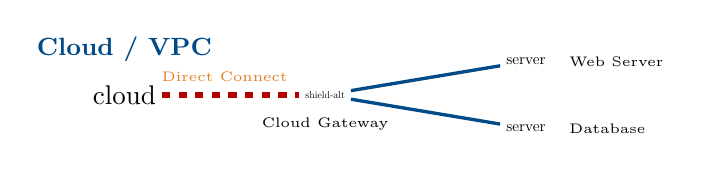
\begin{tikzpicture}[scale=0.85]
            % Cloud
            \node[cloud] (cloud) at (0,0) {\iconcloud[0.8cm]};
            \node[font=\small\bfseries, rctcblue, above=0.1cm of cloud] {Cloud / VPC};
            
            % Gateway
            \node[firewall] (gw) at (3,0) {\iconfirewall[0.5cm]};
            \node[font=\tiny, below=0.05cm of gw] {Cloud Gateway};
            
            % DC
            \node[server] (dc1) at (6,0.5) {\iconserver[0.5cm]};
            \node[server] (dc2) at (6,-0.5) {\iconserver[0.5cm]};
            \node[font=\tiny, right=0.1cm of dc1] {Web Server};
            \node[font=\tiny, right=0.1cm of dc2] {Database};
            
            \draw[alertred, dashed, line width=2pt] (cloud) -- (gw);
            \node[font=\tiny, aborange, above=0.05cm] at (1.5,0) {Direct Connect};
            \draw[ethernet noarrow, line width=1.2pt] (gw) -- (dc1);
            \draw[ethernet noarrow, line width=1.2pt] (gw) -- (dc2);
        \end{tikzpicture}
    \end{center}
\end{frame}

% =============================================================================
% SLIDE 2: Outline
% =============================================================================
\presentationonly{
\begin{frame}[allowframebreaks]{Outline}
\small
\tableofcontents[hideallsubsections]
\end{frame}
}

% =============================================================================
% SLIDE 3: Review
% =============================================================================
\section*{Review from Module 13}
\begin{frame}{Review: VPNs and WANs to Modern Cloud}
    \begin{columns}[T]
        \begin{column}{0.55\textwidth}
            \begin{block}{Key Module 13 Concepts}
                \begin{itemize}
                    \item \textbf{WAN Links} connect geographically separated LANs using ISP infrastructure.
                    \item \textbf{VPNs} provide secure, encrypted tunnels over the public internet.
                    \item \textbf{IPsec} secures IP traffic by encrypting the packet (ESP) and verifying its integrity.
                \end{itemize}
            \end{block}
            \vspace{0.3em}
            \begin{exampleblock}{The Question for Module 14}
                As businesses move away from traditional on-premise servers, how are modern networks designed? How do we securely connect to and manage \textbf{Cloud Resources} and \textbf{Software-Defined Networks}?
            \end{exampleblock}
        \end{column}
        \begin{column}{0.42\textwidth}
            \begin{center}
                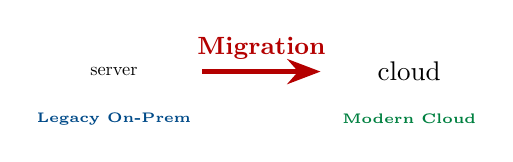
\begin{tikzpicture}[scale=0.75]
                    \node[server] (old) at (0,2) {\iconserver[0.6cm]};
                    \node[font=\tiny\bfseries, rctcblue] at (0,1.2) {Legacy On-Prem};
                    
                    \draw[-{Stealth}, line width=2pt, alertred] (1.5,2) -- (3.5,2);
                    \node[font=\small\bfseries, alertred] at (2.5,2.4) {Migration};
                    
                    \node[cloud] (new) at (5,2) {\iconcloud[0.8cm]};
                    \node[font=\tiny\bfseries, networkgreen] at (5,1.2) {Modern Cloud};
                \end{tikzpicture}
                \par\tiny\textit{The transition from legacy hardware to flexible, cloud-based software-defined networks.}
            \end{center}
        \end{column}
    \end{columns}
\end{frame}

% =============================================================================
% SLIDES 4-5: Learning Outcomes
% =============================================================================
\begin{frame}[t,allowframebreaks]{Learning Outcomes}
    After completing this module, you will be able to:
    \vspace{0.4em}
    \begin{itemize}
        \item Contrast traditional 3-tier data center designs with \keyterm{Spine and Leaf} topologies.
        \item Explain the purpose of a \keyterm{Storage Area Network (SAN)} and contrast \keyterm{Fibre Channel} with \keyterm{iSCSI}.
        \item Differentiate between \keyterm{scalability} (scaling up vs. out) and \keyterm{elasticity}.
        \item Categorize cloud environments by deployment model (Public, Private, Hybrid) and service model (IaaS, PaaS, SaaS).
        \item Describe the function of \keyterm{Content Delivery Networks (CDNs)}.
        \item Identify key cloud networking components: \keyterm{Instances}, \keyterm{VPCs}, and \keyterm{Cloud Gateways}.
        \item Secure cloud networks using \keyterm{Security Groups} and \keyterm{Network ACLs}.
        \item Explain the benefits of \keyterm{Infrastructure as Code (IaC)} and \keyterm{Source Control}.
        \item Describe \keyterm{Software-Defined Networking (SDN)} and the separation of the control plane from the data plane.
        \item Define \keyterm{SD-WAN}, \keyterm{Overlay Networks}, \keyterm{Zero Trust Architecture}, and \keyterm{SASE}.
    \end{itemize}
\end{frame}

% =============================================================================
% SECTION 1: Datacenter and Storage Networks
% =============================================================================
\section{Datacenter and Storage Networks}
\subsection{Data Center Network Design}

\sectionslide{Section 1: Datacenter and Storage Networks}

\begin{frame}[t]{Data Center Network Design}
    \begin{columns}[T]
        \begin{column}{0.48\textwidth}
            \begin{itemize}
                \item Traditional data centers were built using a \keyterm{3-Tier Architecture}: Core, Aggregation (Distribution), and Access.
                \item This design was optimized for \textbf{North-South Traffic}:
                \begin{itemize}
                    \footnotesize
                    \item Traffic flowing from clients (outside) to servers (inside), and vice versa.
                \end{itemize}
                \item \textbf{The Problem:} Modern applications require massive amounts of \textbf{East-West Traffic} (server-to-server communication).
            \end{itemize}
        \end{column}
        \begin{column}{0.5\textwidth}
            \begin{center}
                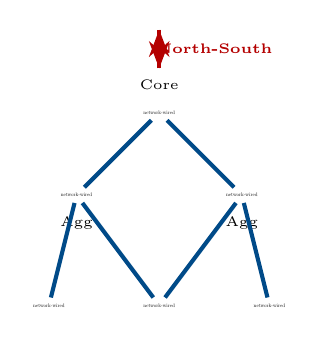
\begin{tikzpicture}[scale=0.7]
                    % Core
                    \node[switch] (c1) at (2,4) {\iconswitch[0.4cm]};
                    \node[font=\tiny] at (2,4.5) {Core};
                    % Agg
                    \node[switch] (ag1) at (0.5,2.5) {\iconswitch[0.4cm]};
                    \node[switch] (ag2) at (3.5,2.5) {\iconswitch[0.4cm]};
                    \node[font=\tiny] at (0.5,2) {Agg};
                    \node[font=\tiny] at (3.5,2) {Agg};
                    % Access
                    \node[switch] (ac1) at (0,0.5) {\iconswitch[0.4cm]};
                    \node[switch] (ac2) at (2,0.5) {\iconswitch[0.4cm]};
                    \node[switch] (ac3) at (4,0.5) {\iconswitch[0.4cm]};
                    
                    \draw[ethernet noarrow] (c1) -- (ag1);
                    \draw[ethernet noarrow] (c1) -- (ag2);
                    \draw[ethernet noarrow] (ag1) -- (ac1);
                    \draw[ethernet noarrow] (ag1) -- (ac2);
                    \draw[ethernet noarrow] (ag2) -- (ac2);
                    \draw[ethernet noarrow] (ag2) -- (ac3);
                    
                    \draw[-{Stealth}, alertred, line width=1.5pt] (2,4.8) -- (2,5.5);
                    \draw[-{Stealth}, alertred, line width=1.5pt] (2,5.5) -- (2,4.8);
                    \node[font=\tiny\bfseries, alertred] at (3,5.15) {North-South};
                \end{tikzpicture}
                \par\tiny\textit{Traditional 3-tier network focusing on North-South flows.}
            \end{center}
        \end{column}
    \end{columns}
\end{frame}

\subsection{Spine and Leaf Topology}
\begin{frame}[t]{Spine and Leaf Topology}
    \begin{columns}[T]
        \begin{column}{0.5\textwidth}
            \begin{itemize}
                \item To solve the East-West traffic bottleneck, modern data centers use a \keyterm{Spine and Leaf} topology.
                \item \textbf{Leaf Switches}: Access switches that connect directly to servers.
                \item \textbf{Spine Switches}: The backbone. \textit{Every leaf switch connects to every spine switch.}
                \item \textbf{Key Benefit}: Consistent latency. Any server is always exactly the same number of hops away from any other server.
            \end{itemize}
        \end{column}
        \begin{column}{0.48\textwidth}
            \begin{center}
                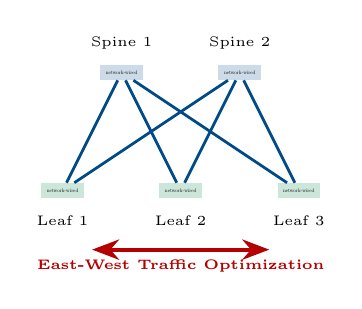
\begin{tikzpicture}[scale=0.75]
                    % Spines
                    \node[switch, fill=rctcblue!20] (sp1) at (1,3) {\iconswitch[0.4cm]};
                    \node[switch, fill=rctcblue!20] (sp2) at (3,3) {\iconswitch[0.4cm]};
                    \node[font=\tiny] at (1,3.5) {Spine 1};
                    \node[font=\tiny] at (3,3.5) {Spine 2};
                    
                    % Leafs
                    \node[switch, fill=networkgreen!20] (lf1) at (0,1) {\iconswitch[0.4cm]};
                    \node[switch, fill=networkgreen!20] (lf2) at (2,1) {\iconswitch[0.4cm]};
                    \node[switch, fill=networkgreen!20] (lf3) at (4,1) {\iconswitch[0.4cm]};
                    \node[font=\tiny, below=0.1cm of lf1] {Leaf 1};
                    \node[font=\tiny, below=0.1cm of lf2] {Leaf 2};
                    \node[font=\tiny, below=0.1cm of lf3] {Leaf 3};
                    
                    % Connections (Every leaf to every spine)
                    \draw[ethernet noarrow, line width=1pt] (lf1) -- (sp1);
                    \draw[ethernet noarrow, line width=1pt] (lf1) -- (sp2);
                    \draw[ethernet noarrow, line width=1pt] (lf2) -- (sp1);
                    \draw[ethernet noarrow, line width=1pt] (lf2) -- (sp2);
                    \draw[ethernet noarrow, line width=1pt] (lf3) -- (sp1);
                    \draw[ethernet noarrow, line width=1pt] (lf3) -- (sp2);
                    
                    % East West Arrow
                    \draw[{Stealth}-{Stealth}, alertred, line width=1.5pt] (0.5,0) -- (3.5,0);
                    \node[font=\tiny\bfseries, alertred, below] at (2,0) {East-West Traffic Optimization};
                \end{tikzpicture}
            \end{center}
        \end{column}
    \end{columns}
\end{frame}

\subsection{Storage Area Networks}
\begin{frame}[t]{Storage Area Networks (SANs)}
    \begin{itemize}
        \item A \keyterm{Storage Area Network (SAN)} is a specialized, high-speed network that provides block-level network access to storage.
        \item It removes the heavy burden of storage traffic from the main LAN.
    \end{itemize}
    \vspace{0.3em}
    \begin{block}{Block Storage vs. File Storage}
        \begin{itemize}
            \footnotesize
            \item \textbf{File Storage (NAS)}: Operates at the file level (like a shared folder via SMB or NFS). The NAS handles the file system.
            \item \textbf{Block Storage (SAN)}: Storage is presented as raw, empty volumes (blocks). The connecting server formats it and treats it as a locally attached hard drive (e.g., the C: drive on Windows).
        \end{itemize}
    \end{block}
\end{frame}

\subsection{Fibre Channel and iSCSI}
\begin{frame}[t]{Fibre Channel (FC)}
    \begin{columns}[T]
        \begin{column}{0.48\textwidth}
            \begin{itemize}
                \item \keyterm{Fibre Channel (FC)} is a purpose-built protocol designed specifically for SANs.
                \item Provides extremely high speeds, low latency, and zero packet loss.
                \item \textbf{Requirements}:
                \begin{itemize}
                    \footnotesize
                    \item Specialized FC switches.
                    \item Fiber optic cabling.
                    \item \keyterm{Host Bus Adapters (HBAs)} installed in the servers.
                \end{itemize}
                \item \textbf{Drawback}: Very expensive and requires separate infrastructure from the Ethernet LAN.
            \end{itemize}
        \end{column}
        \begin{column}{0.48\textwidth}
            \begin{center}
                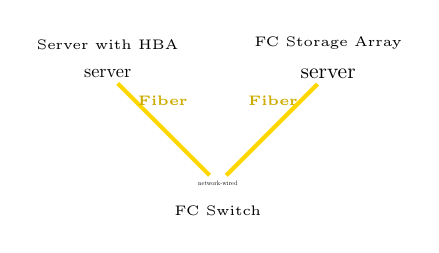
\begin{tikzpicture}[scale=0.7]
                    \node[server] (srv) at (0,2) {\iconserver[0.6cm]};
                    \node[font=\tiny, above=0.05cm of srv] {Server with HBA};
                    
                    \node[switch] (sw) at (2,0) {\iconswitch[0.5cm]};
                    \node[font=\tiny, below=0.05cm of sw] {FC Switch};
                    
                    \node[server] (st) at (4,2) {\iconserver[0.7cm]};
                    \node[font=\tiny, above=0.05cm of st] {FC Storage Array};
                    
                    \draw[fiber noarrow, line width=1.5pt] (srv) -- (sw);
                    \draw[fiber noarrow, line width=1.5pt] (sw) -- (st);
                    
                    \node[font=\tiny\bfseries, fiberyellow!80!black] at (1,1.5) {Fiber};
                    \node[font=\tiny\bfseries, fiberyellow!80!black] at (3,1.5) {Fiber};
                \end{tikzpicture}
                \par\tiny\textit{A dedicated Fibre Channel fabric.}
            \end{center}
        \end{column}
    \end{columns}
\end{frame}

\begin{frame}[t]{iSCSI (Internet Small Computer Systems Interface)}
    \begin{columns}[T]
        \begin{column}{0.5\textwidth}
            \begin{itemize}
                \item \keyterm{iSCSI} encapsulates SCSI storage commands inside standard IP packets.
                \item Runs over standard Ethernet networks (TCP/IP).
                \item \textbf{Benefits}: Cheaper than Fibre Channel because it uses existing Ethernet switches and standard Network Interface Cards (NICs).
                \item \textbf{Terminology}:
                \begin{itemize}
                    \footnotesize
                    \item \keyterm{Initiator}: The server requesting the storage.
                    \item \keyterm{Target}: The storage device providing the disks.
                \end{itemize}
            \end{itemize}
        \end{column}
        \begin{column}{0.45\textwidth}
            \begin{center}
                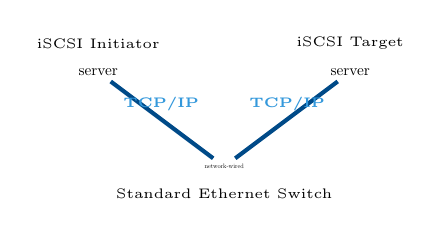
\begin{tikzpicture}[scale=0.8]
                    \node[server] (init) at (0,2) {\iconserver[0.5cm]};
                    \node[font=\tiny, above=0.05cm of init] {iSCSI Initiator};
                    
                    \node[switch] (sw) at (2,0.5) {\iconswitch[0.5cm]};
                    \node[font=\tiny, below=0.05cm of sw] {Standard Ethernet Switch};
                    
                    \node[server] (targ) at (4,2) {\iconserver[0.5cm]};
                    \node[font=\tiny, above=0.05cm of targ] {iSCSI Target};
                    
                    \draw[ethernet noarrow, line width=1.5pt] (init) -- (sw);
                    \draw[ethernet noarrow, line width=1.5pt] (sw) -- (targ);
                    
                    \node[font=\tiny\bfseries, ipblue] at (1,1.5) {TCP/IP};
                    \node[font=\tiny\bfseries, ipblue] at (3,1.5) {TCP/IP};
                \end{tikzpicture}
            \end{center}
        \end{column}
    \end{columns}
\end{frame}

\begin{frame}[t]{Case Study 1: Mercy General Hospital SAN (Problem)}
    \begin{casestudy}{The Problem: Imaging Bottlenecks}
        \footnotesize
        Mercy General Hospital has acquired a new fleet of advanced MRI machines. These machines generate massive, high-resolution 3D imaging files (often over 5GB per scan). 
        
        Currently, the MRI machines save files over the standard LAN to a traditional Network Attached Storage (NAS) file server. Due to heavy daytime network traffic from hospital staff, the MRI machines frequently time out while saving, and doctors face severe lag when trying to load and manipulate the 3D models in the operating room.
    \end{casestudy}
    
    \begin{alertblock}{Challenges}
        \begin{itemize}
            \footnotesize
            \item The standard LAN is congested (East-West and North-South traffic mixed).
            \item The file-level protocol (SMB) adds too much overhead for massive 3D models.
            \item The hospital requires zero packet loss and absolute minimum latency for surgical imaging.
        \end{itemize}
    \end{alertblock}
\end{frame}

\begin{frame}[t]{Case Study 1: Mercy General Hospital SAN (Solution)}
    \begin{casesolution}{The Solution: Dedicated Fibre Channel SAN}
        \footnotesize
        The IT team designs a completely separate, dedicated network solely for storage traffic.
        \begin{itemize}
            \item \textbf{Architecture}: They implement a \keyterm{Storage Area Network (SAN)}.
            \item \textbf{Protocol Choice}: While iSCSI is cheaper, the strict zero-latency and zero-drop requirements push them to select \keyterm{Fibre Channel (FC)}.
            \item \textbf{Hardware}: They install specialized FC switches, run fiber optic cables, and install Host Bus Adapters (HBAs) in the imaging servers.
            \item \textbf{Outcome}: The storage arrays now appear as local, high-speed block storage. Storage traffic no longer competes with hospital LAN traffic. Doctors can instantly load MRI models, and saves happen instantaneously without timeouts.
        \end{itemize}
    \end{casesolution}
\end{frame}


% =============================================================================
% SECTION 2: Cloud Concepts
% =============================================================================
\section{Cloud Concepts}
\subsection{Cloud Scalability and Elasticity}

\sectionslide{Section 2: Cloud Concepts}

\begin{frame}[t]{What is Cloud Computing?}
    \begin{itemize}
        \item \textbf{Cloud Computing} is the on-demand delivery of IT resources over the internet with pay-as-you-go pricing.
        \item Instead of buying, owning, and maintaining physical data centers, you access technology services (computing power, storage, databases) on an as-needed basis.
    \end{itemize}
    \vspace{0.4em}
    \begin{block}{Five Essential Characteristics (NIST)}
        \begin{enumerate}
            \footnotesize
            \item On-demand self-service
            \item Broad network access
            \item Resource pooling (Multi-tenancy)
            \item Rapid elasticity
            \item Measured service (Pay-as-you-go)
        \end{enumerate}
    \end{block}
\end{frame}

\begin{frame}[t]{Scalability: Scale Up vs. Scale Out}
    \begin{columns}[T]
        \begin{column}{0.48\textwidth}
            \begin{block}{\keyterm{Scale Up} (Vertical Scaling)}
                \footnotesize
                \begin{itemize}
                    \item Adding more resources to an \textit{existing} server (e.g., adding more RAM, upgrading the CPU).
                    \item \textbf{Pros}: Easy to implement, application doesn't need to change.
                    \item \textbf{Cons}: Hardware limits (you can only get so big), requires downtime.
                \end{itemize}
            \end{block}
        \end{column}
        \begin{column}{0.48\textwidth}
            \begin{block}{\keyterm{Scale Out} (Horizontal Scaling)}
                \footnotesize
                \begin{itemize}
                    \item Adding \textit{more servers} to a pool or cluster (e.g., adding 5 more web servers behind a load balancer).
                    \item \textbf{Pros}: Virtually limitless, provides high availability.
                    \item \textbf{Cons}: Requires software designed for distributed computing.
                \end{itemize}
            \end{block}
        \end{column}
    \end{columns}
\end{frame}

\begin{frame}[t]{Elasticity}
    \begin{itemize}
        \item \keyterm{Elasticity} is the ability of the cloud to \textit{automatically} scale resources \textbf{up AND down} dynamically based on current demand.
        \item This ensures you always have enough capacity during spikes, but you aren't paying for idle servers during quiet periods.
    \end{itemize}
    \vspace{0.2em}
    \begin{center}
        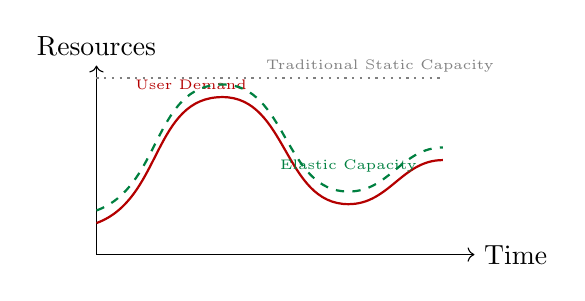
\begin{tikzpicture}[scale=0.8]
            % Axis
            \draw[->] (0,0) -- (6,0) node[right] {Time};
            \draw[->] (0,0) -- (0,3) node[above] {Resources};
            
            % Demand curve
            \draw[thick, alertred] (0,0.5) to[out=20,in=180] (2,2.5) to[out=0,in=180] (4,0.8) to[out=0,in=180] (5.5,1.5);
            \node[font=\tiny, alertred] at (1.5,2.7) {User Demand};
            
            % Capacity curve (elastic)
            \draw[thick, networkgreen, dashed] (0,0.7) to[out=20,in=180] (2,2.7) to[out=0,in=180] (4,1.0) to[out=0,in=180] (5.5,1.7);
            \node[font=\tiny, networkgreen] at (4,1.4) {Elastic Capacity};
            
            % Static capacity line
            \draw[thick, gray, dotted] (0,2.8) -- (5.5,2.8);
            \node[font=\tiny, gray] at (4.5,3.0) {Traditional Static Capacity};
        \end{tikzpicture}
        \par\tiny\textit{Elasticity matches capacity closely to demand, avoiding the wasted cost of static over-provisioning.}
    \end{center}
\end{frame}

\subsection{Cloud Deployment Models}
\begin{frame}[t]{Cloud Deployment Models}
    \begin{columns}[T]
        \begin{column}{0.48\textwidth}
            \begin{block}{\keyterm{Public Cloud}}
                \footnotesize
                \begin{itemize}
                    \item Services are offered over the public internet and available to anyone who wants to purchase them.
                    \item Owned and operated by a third-party provider (AWS, Microsoft Azure, Google Cloud).
                    \item \textbf{Pros}: Zero capital expense, massive scale.
                    \item \textbf{Cons}: Less control, multi-tenant environment.
                \end{itemize}
            \end{block}
        \end{column}
        \begin{column}{0.48\textwidth}
            \begin{block}{\keyterm{Private Cloud}}
                \footnotesize
                \begin{itemize}
                    \item Cloud infrastructure operated solely for a \textit{single organization}.
                    \item Can be hosted on-premises or by a third-party provider.
                    \item \textbf{Pros}: Maximum control, security, and strict compliance.
                    \item \textbf{Cons}: High capital expense, responsible for your own maintenance.
                \end{itemize}
            \end{block}
        \end{column}
    \end{columns}
\end{frame}

\begin{frame}[t]{Hybrid and Community Clouds}
    \begin{columns}[T]
        \begin{column}{0.48\textwidth}
            \begin{block}{\keyterm{Hybrid Cloud}}
                \footnotesize
                \begin{itemize}
                    \item A combination of Public and Private clouds, connected by secure technology (like a VPN or Direct Connect) that allows data and applications to be shared between them.
                    \item \textbf{Example}: Keeping sensitive patient data on a Private Cloud while running the web front-end on a Public Cloud.
                \end{itemize}
            \end{block}
        \end{column}
        \begin{column}{0.48\textwidth}
            \begin{block}{\keyterm{Community Cloud}}
                \footnotesize
                \begin{itemize}
                    \item Infrastructure shared by several organizations with common concerns (e.g., security, compliance, jurisdiction).
                    \item \textbf{Example}: Multiple local government agencies sharing a cloud infrastructure specifically built for government compliance.
                \end{itemize}
            \end{block}
        \end{column}
    \end{columns}
\end{frame}

\subsection{Cloud Service Models}
\begin{frame}[t]{Cloud Service Models: IaaS, PaaS, SaaS}
    \begin{center}
        \footnotesize
        \begin{tabular}{l l p{6.5cm}}
            \toprule
            \textbf{Model} & \textbf{What You Manage} & \textbf{Examples} \\
            \midrule
            \rowcolor{ipblue!15}
            \keyterm{IaaS} & OS, Data, Apps, Runtime & AWS EC2, Azure VMs \\
            \rowcolor{networkgreen!15}
            \keyterm{PaaS} & Data, Apps & AWS Elastic Beanstalk, Heroku \\
            \rowcolor{rctcblue!10}
            \keyterm{SaaS} & Nothing (Just use it) & Office 365, Salesforce, Gmail \\
            \bottomrule
        \end{tabular}
    \end{center}
    
    \vspace{0.4em}
    \begin{block}{The Pizza as a Service Analogy}
        \footnotesize
        \begin{itemize}
            \item \textbf{On-Premises}: You make the pizza from scratch at home.
            \item \textbf{IaaS}: Take-and-bake. You buy the pre-made pizza, but you bake it in your oven and set the table.
            \item \textbf{PaaS}: Delivery. They cook and deliver it; you just eat it at your table.
            \item \textbf{SaaS}: Dining out. The restaurant does everything; you just sit and eat.
        \end{itemize}
    \end{block}
\end{frame}

\subsection{Content Delivery Networks}
\begin{frame}[t]{Content Delivery Networks (CDNs)}
    \begin{columns}[T]
        \begin{column}{0.5\textwidth}
            \begin{itemize}
                \item A \keyterm{CDN} is a geographically distributed network of proxy servers and their data centers.
                \item \textbf{Goal}: Provide high availability and performance by distributing the service spatially relative to end-users.
                \item \textbf{How it works}: Static assets (images, videos, HTML) are cached on "Edge Servers" near the user.
                \item Drastically reduces latency and offloads traffic from the origin server.
            \end{itemize}
        \end{column}
        \begin{column}{0.45\textwidth}
            \begin{center}
                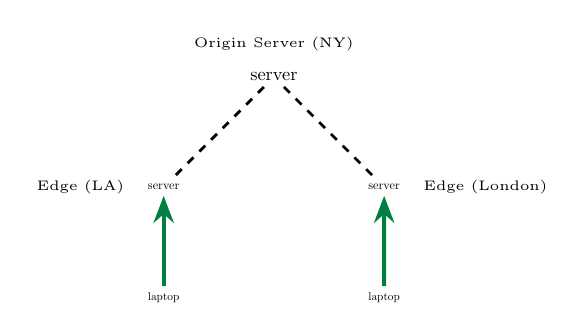
\begin{tikzpicture}[scale=0.7]
                    \node[server] (origin) at (2,4) {\iconserver[0.6cm]};
                    \node[font=\tiny] at (2,4.6) {Origin Server (NY)};
                    
                    \node[server] (edge1) at (0,2) {\iconserver[0.4cm]};
                    \node[server] (edge2) at (4,2) {\iconserver[0.4cm]};
                    \node[font=\tiny, left=0.1cm of edge1] {Edge (LA)};
                    \node[font=\tiny, right=0.1cm of edge2] {Edge (London)};
                    
                    \node[laptop] (u1) at (0,0) {\iconlaptop[0.4cm]};
                    \node[laptop] (u2) at (4,0) {\iconlaptop[0.4cm]};
                    
                    \draw[dashed, line width=1pt] (origin) -- (edge1);
                    \draw[dashed, line width=1pt] (origin) -- (edge2);
                    
                    \draw[-{Stealth}, networkgreen, line width=1.5pt] (u1) -- (edge1);
                    \draw[-{Stealth}, networkgreen, line width=1.5pt] (u2) -- (edge2);
                \end{tikzpicture}
                \par\tiny\textit{Users pull content from local Edge Servers rather than crossing the globe to the Origin Server.}
            \end{center}
        \end{column}
    \end{columns}
\end{frame}

\begin{frame}[t]{Case Study 2: Mercy General Hospital Hybrid Cloud (Problem)}
    \begin{casestudy}{The Problem: Seasonal Traffic Surges}
        \footnotesize
        Mercy General Hospital operates a web-based Patient Portal where patients can schedule appointments, pay bills, and watch pre-surgery instructional videos. 
        
        During flu season, traffic to the portal spikes by 500\%. The on-premises web servers crash under the load, preventing patients from accessing critical services. Furthermore, patients complaining of slow load times for the heavy instructional videos are overwhelming the IT helpdesk. 
        
        The hospital wants to move to the cloud to handle the load, but strict HIPAA regulations require the actual patient database to remain on physical servers owned and located within the hospital's walls.
    \end{casestudy}
\end{frame}

\begin{frame}[t]{Case Study 2: Mercy General Hospital Hybrid Cloud (Solution)}
    \begin{casesolution}{The Solution: Hybrid Cloud and CDN}
        \footnotesize
        \begin{itemize}
            \item \textbf{Deployment Model}: They adopt a \keyterm{Hybrid Cloud} architecture. The sensitive patient database remains on-premises in their Private Cloud. The web front-end servers are migrated to AWS (Public Cloud).
            \item \textbf{Elasticity}: In AWS, they configure an Auto-Scaling Group. When flu season hits, the cloud \textit{elastically} adds more web servers to handle the load, and automatically removes them when demand drops.
            \item \textbf{Content Delivery Network (CDN)}: They move all heavy instructional videos to a \keyterm{CDN}. Now, patients load videos from Edge Servers located in their own cities, drastically reducing load times and removing the burden from the hospital's origin servers.
        \end{itemize}
    \end{casesolution}
\end{frame}

% =============================================================================
% SECTION 3: Cloud Networking
% =============================================================================
\section{Cloud Networking}
\subsection{Cloud Instances and VPCs}

\sectionslide{Section 3: Cloud Networking}

\begin{frame}[t]{Cloud Instances and VPCs}
    \begin{columns}[T]
        \begin{column}{0.48\textwidth}
            \begin{block}{Cloud Instances}
                \footnotesize
                \begin{itemize}
                    \item A \keyterm{Cloud Instance} is simply a virtual machine (VM) running in a cloud provider's data center (e.g., AWS EC2 instance, Azure VM).
                \end{itemize}
            \end{block}
            \vspace{0.2em}
            \begin{block}{Virtual Private Cloud (VPC)}
                \footnotesize
                \begin{itemize}
                    \item A \keyterm{VPC} is a logically isolated virtual network within a public cloud.
                    \item You define the IP address space (CIDR block), create subnets, configure route tables, and manage network gateways.
                    \item It acts as your own private data center in the cloud.
                \end{itemize}
            \end{block}
        \end{column}
        \begin{column}{0.48\textwidth}
            \begin{center}
                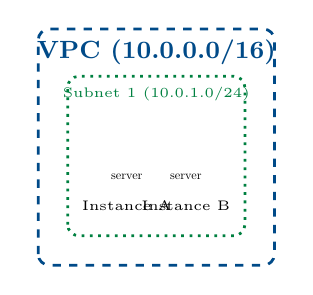
\begin{tikzpicture}[scale=0.75]
                    % VPC boundary
                    \draw[dashed, rctcblue, rounded corners, line width=1pt] (0,0) rectangle (4,4);
                    \node[font=\small\bfseries, rctcblue] at (2,3.6) {VPC (10.0.0.0/16)};
                    
                    % Subnet
                    \draw[dotted, networkgreen, rounded corners, line width=1pt] (0.5,0.5) rectangle (3.5,3.2);
                    \node[font=\tiny, networkgreen] at (2,2.9) {Subnet 1 (10.0.1.0/24)};
                    
                    % Instance
                    \node[server] (inst1) at (1.5,1.5) {\iconserver[0.4cm]};
                    \node[server] (inst2) at (2.5,1.5) {\iconserver[0.4cm]};
                    \node[font=\tiny] at (1.5,1) {Instance A};
                    \node[font=\tiny] at (2.5,1) {Instance B};
                \end{tikzpicture}
            \end{center}
        \end{column}
    \end{columns}
\end{frame}

\subsection{Cloud Gateways and Connectivity}
\begin{frame}[t]{Cloud Gateways}
    \begin{itemize}
        \item For instances in a VPC to communicate outside the VPC, they need a \keyterm{Gateway}.
    \end{itemize}
    \vspace{0.3em}
    \begin{columns}[T]
        \begin{column}{0.48\textwidth}
            \begin{block}{Internet Gateway (IGW)}
                \footnotesize
                \begin{itemize}
                    \item Allows communication between instances in your VPC and the internet.
                    \item Instances must be in a \textit{Public Subnet} and have a public IP address.
                \end{itemize}
            \end{block}
        \end{column}
        \begin{column}{0.48\textwidth}
            \begin{block}{NAT Gateway}
                \footnotesize
                \begin{itemize}
                    \item Allows instances in a \textit{Private Subnet} to access the internet (e.g., for software updates), but prevents the internet from initiating connections back to those instances.
                \end{itemize}
            \end{block}
        \end{column}
    \end{columns}
\end{frame}

\begin{frame}[t]{Cloud Connectivity Options}
    \begin{itemize}
        \item How do you connect your on-premises office network to your Cloud VPC?
    \end{itemize}
    \vspace{0.3em}
    \begin{columns}[T]
        \begin{column}{0.48\textwidth}
            \begin{block}{Site-to-Site VPN}
                \footnotesize
                \begin{itemize}
                    \item Creates an encrypted IPsec tunnel over the \textbf{public internet}.
                    \item \textbf{Pros}: Quick to set up, cost-effective.
                    \item \textbf{Cons}: Subject to internet congestion and variable latency.
                \end{itemize}
            \end{block}
        \end{column}
        \begin{column}{0.48\textwidth}
            \begin{block}{Direct Connection}
                \footnotesize
                \begin{itemize}
                    \item A \textbf{dedicated, private physical network connection} from your office directly to the cloud provider (e.g., AWS Direct Connect, Azure ExpressRoute).
                    \item \textbf{Pros}: Bypasses the internet, guaranteed bandwidth, consistent latency.
                    \item \textbf{Cons}: Expensive, takes weeks/months to install physical lines.
                \end{itemize}
            \end{block}
        \end{column}
    \end{columns}
\end{frame}

\subsection{Cloud Firewall Security}
\begin{frame}[t]{Cloud Firewall Security}
    \begin{itemize}
        \item In the cloud, network security is software-defined rather than relying on physical firewall appliances.
        \item Cloud providers use a two-layered defense system.
    \end{itemize}
    \vspace{0.3em}
    \begin{center}
        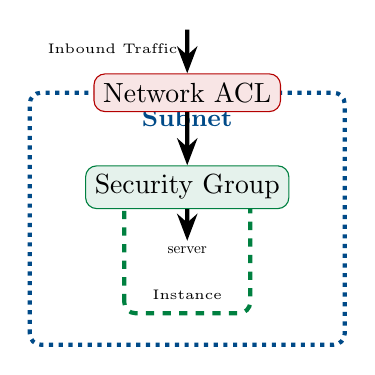
\begin{tikzpicture}[scale=0.8]
            % Subnet boundary
            \draw[dotted, rctcblue, rounded corners, line width=1.5pt] (0,0) rectangle (5,4);
            \node[font=\small\bfseries, rctcblue] at (2.5,3.6) {Subnet};
            
            % Network ACL
            \node[draw=alertred, fill=alertred!10, rounded corners, minimum width=2cm] (nacl) at (2.5,4) {Network ACL};
            
            % Instance boundary
            \draw[dashed, networkgreen, rounded corners, line width=1.5pt] (1.5,0.5) rectangle (3.5,2.5);
            
            % Security Group
            \node[draw=networkgreen, fill=networkgreen!10, rounded corners, minimum width=2cm] (sg) at (2.5,2.5) {Security Group};
            
            % Instance
            \node[server] (inst) at (2.5,1.5) {\iconserver[0.5cm]};
            \node[font=\tiny] at (2.5,0.8) {Instance};
            
            % Traffic arrow
            \draw[-{Stealth}, line width=1.5pt] (2.5,5) -- (nacl);
            \draw[-{Stealth}, line width=1.5pt] (nacl) -- (sg);
            \draw[-{Stealth}, line width=1.5pt] (sg) -- (inst);
            \node[font=\tiny, left] at (2.5,4.7) {Inbound Traffic};
        \end{tikzpicture}
    \end{center}
\end{frame}

\begin{frame}[t]{Security Groups vs. Network ACLs}
    \begin{columns}[T]
        \begin{column}{0.48\textwidth}
            \begin{block}{\keyterm{Security Groups}}
                \footnotesize
                \begin{itemize}
                    \item Operate at the \textbf{Instance (VM) level}.
                    \item \textbf{Stateful}: If you allow an incoming request (e.g., HTTP on port 80), the return traffic is automatically allowed, regardless of outbound rules.
                    \item Default behavior: Deny all inbound, allow all outbound.
                    \item You specify \textit{allow} rules; you cannot create \textit{deny} rules.
                \end{itemize}
            \end{block}
        \end{column}
        \begin{column}{0.48\textwidth}
            \begin{block}{\keyterm{Network ACLs} (Security Lists)}
                \footnotesize
                \begin{itemize}
                    \item Operate at the \textbf{Subnet level}.
                    \item \textbf{Stateless}: Return traffic must be explicitly allowed by rules. If you allow inbound HTTP on 80, you must explicitly allow outbound traffic on ephemeral ports.
                    \item Support both \textit{allow} and \textit{deny} rules.
                    \item Used as an extra layer of defense around the subnet perimeter.
                \end{itemize}
            \end{block}
        \end{column}
    \end{columns}
\end{frame}

% =============================================================================
% SECTION 4: Modern Network Environments
% =============================================================================
\section{Modern Network Environments}
\subsection{Infrastructure as Code}

\sectionslide{Section 4: Modern Network Environments}

\begin{frame}[t]{Infrastructure as Code (IaC)}
    \begin{columns}[T]
        \begin{column}{0.5\textwidth}
            \begin{itemize}
                \item Traditionally, network admins logged into switches via CLI and typed commands, or clicked through web interfaces to build servers.
                \item \keyterm{Infrastructure as Code (IaC)} is the process of managing and provisioning data centers through \textbf{machine-readable definition files} (code).
                \item Examples: Terraform, AWS CloudFormation, Ansible.
            \end{itemize}
        \end{column}
        \begin{column}{0.48\textwidth}
            \begin{block}{Benefits of IaC}
                \footnotesize
                \begin{itemize}
                    \item \textbf{Consistency}: The code deploys the exact same environment every time, preventing configuration drift.
                    \item \textbf{Speed}: You can deploy 100 servers and a VPC in minutes automatically.
                    \item \textbf{Documentation}: The code serves as live, accurate documentation of your infrastructure.
                \end{itemize}
            \end{block}
        \end{column}
    \end{columns}
\end{frame}

\begin{frame}[t]{Source Control}
    \begin{itemize}
        \item Because infrastructure is now written as code, network engineers must use software development practices.
        \item \keyterm{Source Control} (or Version Control) systems, like \textbf{Git}, track changes to code over time.
    \end{itemize}
    \vspace{0.3em}
    \begin{block}{Why use Source Control for IaC?}
        \footnotesize
        \begin{itemize}
            \item \textbf{History \& Rollbacks}: If a new network configuration breaks production, you can instantly revert the code to the previous working version.
            \item \textbf{Peer Review}: Changes are submitted as "Pull Requests" so other engineers can review the configuration before it is applied.
            \item \textbf{Collaboration}: Multiple engineers can work on the infrastructure codebase simultaneously without overwriting each other's work.
        \end{itemize}
    \end{block}
\end{frame}

\subsection{Software-Defined Networking}
\begin{frame}[t]{Software-Defined Networking (SDN)}
    \begin{columns}[T]
        \begin{column}{0.48\textwidth}
            \begin{itemize}
                \item \keyterm{SDN} shifts networking from hardware-centric to software-centric.
                \item It physically separates the network's \textbf{Control Plane} from the \textbf{Data Plane}.
                \item \textbf{Control Plane}: The "brains." Makes decisions about where traffic should go (routing tables, policies).
                \item \textbf{Data Plane}: The "brawn." Actually moves the packets based on the control plane's instructions.
            \end{itemize}
        \end{column}
        \begin{column}{0.48\textwidth}
            \begin{center}
                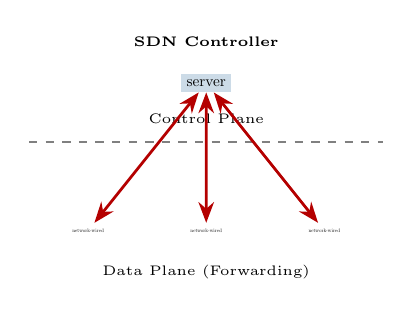
\begin{tikzpicture}[scale=0.75]
                    % Controller
                    \node[server, fill=rctcblue!20] (ctrl) at (2,3.5) {\iconserver[0.5cm]};
                    \node[font=\tiny\bfseries] at (2,4.2) {SDN Controller};
                    \node[font=\tiny] at (2,2.9) {Control Plane};
                    
                    % Line
                    \draw[dashed, gray, line width=1pt] (-1,2.5) -- (5,2.5);
                    
                    % Switches
                    \node[switch] (sw1) at (0,1) {\iconswitch[0.4cm]};
                    \node[switch] (sw2) at (2,1) {\iconswitch[0.4cm]};
                    \node[switch] (sw3) at (4,1) {\iconswitch[0.4cm]};
                    \node[font=\tiny] at (2,0.3) {Data Plane (Forwarding)};
                    
                    % Connections
                    \draw[{Stealth}-{Stealth}, alertred, line width=1pt] (ctrl) -- (sw1);
                    \draw[{Stealth}-{Stealth}, alertred, line width=1pt] (ctrl) -- (sw2);
                    \draw[{Stealth}-{Stealth}, alertred, line width=1pt] (ctrl) -- (sw3);
                \end{tikzpicture}
                \par\tiny\textit{A central controller makes routing decisions and pushes rules down to dumb forwarding switches.}
            \end{center}
        \end{column}
    \end{columns}
\end{frame}

\subsection{SD-WAN and Overlay Networks}
\begin{frame}[t]{Software-Defined WAN (SD-WAN)}
    \begin{itemize}
        \item \keyterm{SD-WAN} applies the principles of SDN to Wide Area Networks.
        \item Traditional WANs relied on expensive, dedicated MPLS circuits. SD-WAN aggregates multiple transport links (e.g., MPLS, Broadband Internet, 5G Cellular) and treats them as a single logical connection.
    \end{itemize}
    \vspace{0.3em}
    \begin{block}{Dynamic Path Selection}
        \footnotesize
        The SD-WAN controller continuously monitors the health of all links (latency, jitter, packet loss). It \textit{dynamically steers traffic} based on application needs.
        \begin{itemize}
            \item \textbf{Example}: Real-time VoIP traffic is automatically routed over the stable MPLS link. If MPLS degrades, VoIP seamlessly shifts to Broadband. Bulk file transfers are sent over the cheaper Broadband link.
        \end{itemize}
    \end{block}
\end{frame}

\begin{frame}[t]{Overlay Networks}
    \begin{itemize}
        \item \keyterm{Overlay Networks} are virtual networks logically built on top of an underlying physical network infrastructure (the \textit{underlay}).
        \item The physical routers just see standard IP packets, but inside those packets are encapsulated virtual network frames.
    \end{itemize}
    \vspace{0.3em}
    \begin{block}{Example: VXLAN}
        \footnotesize
        \begin{itemize}
            \item \textbf{VXLAN} (Virtual Extensible LAN) is an overlay technology used heavily in modern data centers.
            \item It encapsulates Layer 2 Ethernet frames inside Layer 3 UDP packets.
            \item \textbf{Why?}: It allows a Layer 2 network to stretch across Layer 3 boundaries. You can have VMs in completely different physical data centers acting like they are plugged into the exact same local switch.
        \end{itemize}
    \end{block}
\end{frame}

\subsection{Zero Trust and SASE}
\begin{frame}[t]{Zero Trust Architecture (ZTA)}
    \begin{columns}[T]
        \begin{column}{0.48\textwidth}
            \begin{itemize}
                \item \textbf{Legacy Security}: "Trust but verify." Once a user connected to the VPN, they were inside the "trusted" perimeter and had broad network access.
                \item \keyterm{Zero Trust Architecture}: "Never trust, always verify." Assumes the network is already compromised.
            \end{itemize}
        \end{column}
        \begin{column}{0.48\textwidth}
            \begin{block}{Zero Trust Principles}
                \footnotesize
                \begin{itemize}
                    \item \textbf{No Implicit Trust}: Being on the corporate network grants zero privileges.
                    \item \textbf{Continuous Verification}: Identity, device health, and location are authenticated for \textit{every single access request}.
                    \item \textbf{Least Privilege}: Users only get access to the specific app they need, not the whole network.
                \end{itemize}
            \end{block}
        \end{column}
    \end{columns}
\end{frame}

\begin{frame}[t]{Secure Access Service Edge (SASE)}
    \begin{itemize}
        \item \keyterm{SASE} (pronounced "sassy") is a cloud architecture model that bundles \textbf{SD-WAN} capabilities with \textbf{Cloud-Native Security} (including Zero Trust).
        \item Instead of routing remote user traffic back to a corporate data center firewall (tromboning), traffic is inspected in the cloud, close to the user.
    \end{itemize}
    \vspace{0.3em}
    \begin{center}
        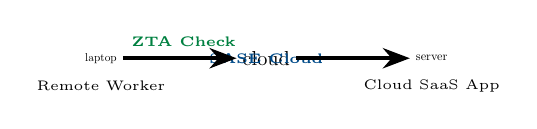
\begin{tikzpicture}[scale=0.7]
            \node[laptop] (user) at (0,2) {\iconlaptop[0.4cm]};
            \node[font=\tiny] at (0,1.5) {Remote Worker};
            
            \node[cloud] (sase) at (3,2) {\iconcloud[0.6cm]};
            \node[font=\tiny\bfseries, rctcblue] at (3,2) {SASE Cloud};
            
            \node[server] (app) at (6,2) {\iconserver[0.4cm]};
            \node[font=\tiny] at (6,1.5) {Cloud SaaS App};
            
            \draw[-{Stealth}, line width=1.5pt] (user) -- (sase);
            \draw[-{Stealth}, line width=1.5pt] (sase) -- (app);
            \node[font=\tiny\bfseries, networkgreen] at (1.5,2.3) {ZTA Check};
        \end{tikzpicture}
        \par\tiny\textit{SASE moves security enforcement to the cloud edge, verifying access before forwarding to the application.}
    \end{center}
\end{frame}

\begin{frame}[t]{Case Study 3: Mercy General Hospital SD-WAN (Problem)}
    \begin{casestudy}{The Problem: Unreliable Telemedicine and Legacy VPNs}
        \footnotesize
        Mercy General employs hundreds of remote doctors performing telemedicine video calls from home. The video calls frequently drop because standard residential broadband is unreliable. 
        
        Additionally, to access patient records, doctors use a legacy VPN. Once connected, their personal laptops have broad access to the hospital's internal network. Last month, malware from a doctor's compromised home PC traveled through the VPN tunnel and infected a hospital file server.
    \end{casestudy}
    
    \begin{alertblock}{Challenges}
        \begin{itemize}
            \footnotesize
            \item Unreliable single-link home internet causes dropped video calls.
            \item Legacy VPN provides too much "trusted" access to the internal network.
            \item Need a way to secure access without routing all traffic through a central choke point.
        \end{itemize}
    \end{alertblock}
\end{frame}

\begin{frame}[t]{Case Study 3: Mercy General Hospital SD-WAN (Solution)}
    \begin{casesolution}{The Solution: SD-WAN and Zero Trust (SASE)}
        \footnotesize
        \begin{itemize}
            \item \textbf{SD-WAN at Home}: Doctors are issued small \keyterm{SD-WAN} routers. They plug in their broadband connection and a 5G cellular modem. The SD-WAN actively monitors link health and steers the telemedicine video packets over the healthiest link, eliminating drops.
            \item \textbf{Zero Trust Architecture}: The legacy VPN is retired. They adopt a \keyterm{SASE} model. 
            \item \textbf{Outcome}: Being connected to the internet no longer grants access to the hospital LAN. When a doctor requests a patient record, the SASE cloud performs a \textbf{Continuous Verification} check—ensuring the doctor's identity and that their laptop's antivirus is active—before granting access to \textit{only} the records application, not the whole network.
        \end{itemize}
    \end{casesolution}
\end{frame}

\end{document}
